\documentclass[3p,twocolumn,authoryear]{elsarticle}

\usepackage{natbib}
\usepackage{algorithm}
\usepackage{algpseudocode}
\usepackage{booktabs}
\usepackage{graphicx}
\usepackage{amsmath}
%% \usepackage{lineno}

\journal{Artificial Intelligence in Agriculture}
\bibliographystyle{elsarticle-harv}

\begin{document}
\begin{frontmatter}

\title{Cluster-Conditioned SHAP for Interpretable Allocation Systems:
       Methodology and Agricultural Extension Application}

\author[inst1]{Kitti Chiewchan\corref{cor1}}
\ead{kitti.ch@bsru.ac.th}
\author[inst2]{Jumtip Seneerattanaprayul}

\cortext[cor1]{Corresponding author}
\address[inst1]{Computer Education Program, Faculty of Education,
  Bansomdejchaopraya Rajabhat University,
  1061 Issaraphap Road, Hirunrujee, Thonburi, Bangkok 10600, Thailand}
\address[inst2]{Department of Agricultural and Resource Economics,
  Faculty of Economics, Kasetsart University,
  50 Ngam Wong Wan Road, Ladyao, Jatujak, Bangkok 10110, Thailand}

\begin{abstract}
Allocating interventions to heterogeneous populations requires interpretable decision logic that captures non-linear effects and reveals which characteristics drive differential outcomes. We propose SAR (Segment--Attribute--Recommend), a cluster-conditioned explainable AI framework that integrates K-Means clustering, Random Forest regression, and SHapley Additive exPlanations (SHAP) into a unified pipeline for transparent, rule-based allocation decisions. SAR computes feature importance separately within population clusters and converts cluster-specific SHAP attributions into actionable IF--THEN rules via surrogate decision trees. The approach is general and transferable across domains requiring interpretable resource allocation.

We demonstrate SAR on agricultural skill development using panel survey data from $n=833$ farmers in Thailand's Smart Farmer program. The framework identifies three farmer segments with systematically different determinants of skill improvement: baseline capability, production management competency, and educational attainment. Surrogate rules achieve 91.4\% held-out validation accuracy (80/20 farmer-level split), 95.3\% $\pm$ 2.5\% cross-validated accuracy, and 93.3\% in-sample fidelity.

SAR offers a practical, auditable, and human-centered framework for interpretable allocation in educational, healthcare, and human resources contexts. The approach bridges a gap in explainable AI: translating SHAP-based attribution into operational decision structures that practitioners can apply without technical expertise. Results are subject to population-specific recalibration.
\end{abstract}

\begin{keyword}
Explainable AI \sep SHAP \sep Cluster-Stratified Attribution \sep 
Interpretability \sep Decision Rules \sep Resource Allocation \sep 
Human Capital Development
\end{keyword}

\end{frontmatter}

%% \linenumbers

\section{Introduction}

Allocating interventions---training programs, resources, policy treatments---to heterogeneous populations is a central challenge across multiple domains. This problem appears in education (matching students to instructional methods suited to their prior knowledge), healthcare (stratifying patients for treatment selection), human resources (assigning workers to development tracks), and agricultural extension (matching farmers to training programs). In each context, effective allocation requires more than predictive accuracy; it demands interpretable decision logic that reveals which characteristics of individuals drive differential outcomes. Black-box models fail this requirement: practitioners in resource-constrained settings need transparent, auditable rules they can apply and defend to stakeholders.

In agricultural extension specifically, the allocation problem is acute. Farmers differ widely in baseline skills, resource access, risk perception, and readiness to learn. Yet most national extension systems still rely on standardized curricula \citep{anderson2004,feder1985}, leading to uneven outcomes and inefficient resource use. Precision allocation---matching farmers to training programs suited to their current capability and constraints---could improve program effectiveness. However, such allocation requires not only models that predict training outcomes but decision structures that explain \textit{why} recommendations differ across farmer groups.

Explainable AI (XAI), particularly SHapley Additive exPlanations (SHAP), offers a principled approach to feature attribution grounded in cooperative game theory \citep{lundberg2017}. SHAP-based methods have been applied across domains to explain predictions and support interpretability \citep{arrieta2020,lundberg2020}. In agriculture, SHAP has been used for yield prediction, disease diagnosis, and risk assessment \citep{ghosal2018,ryo2022}. However, two gaps remain. First, most XAI applications stop at post-hoc interpretation and do not translate explanations into operational decision rules \citep{ryo2022,linardatos2021}. Second, they typically compute global feature importance, which obscures a critical insight: the determinants of outcomes often differ systematically across population segments. A feature driving outcomes in one segment may be irrelevant in another, yet standard global attribution methods hide this heterogeneity.

This study proposes \textbf{SAR (Segment--Attribute--Recommend)}, a cluster-conditioned explainable AI framework that addresses these gaps. SAR integrates K-Means clustering, Random Forest regression, and cluster-stratified SHAP analysis into a unified pipeline that extracts transparent, segment-specific decision rules via surrogate decision trees. The framework is general and transferable; we demonstrate it on agricultural skill allocation, but the approach applies to any domain requiring interpretable resource allocation. SAR's novelty does not lie in its individual components---K-Means, Random Forest, and SHAP are well-established methods---but in how they are combined into a unified pipeline that converts cluster-conditioned attribution into practical decision support. To the authors' knowledge, this is the first framework to integrate cluster-stratified SHAP analysis with surrogate rule extraction for allocation decisions.

\section{Literature Review}
%%─────────────────────────────────────────────────────────────────────────────

\subsection{Machine Learning and Computer Vision in Agriculture}

Machine learning and computer vision now play a central role in modern precision
agriculture. They support tasks such as crop monitoring, disease detection,
yield estimation, and livestock identification. \citet{ghazal2024survey} show
that image-based sensing remains the dominant approach across the crop
production cycle. CNN-based models often outperform classical ML for cattle
identification when sufficient training data are available \citep{hossain2022cattle}.
Random Forest and deep learning models are also widely used for nutrient
prediction \citep{ennaji2023nutrient}. For plant disease detection, deep
learning does not always outperform classical ML, highlighting the importance of
selecting methods based on data characteristics \citep{omaye2024disease}. ML has
also improved practical tasks such as quality inspection and grading in
production systems \citep{wonggasem2024}.

Overall, these studies demonstrate strong progress in perception-focused
applications but also reveal limited integration with downstream decision-making.
This gap motivates the need for frameworks that go beyond sensing tasks and
provide interpretable, actionable guidance for practitioners.

\subsection{Explainable AI for Agricultural Decision Support}

As ML models become more complex, explainable AI (XAI) has become essential for
transparency and accountability in agricultural systems
\citep{arrieta2020,linardatos2021}. \citet{guidotti2019} provide a taxonomy of
explanation methods, including feature attribution, surrogate modelling, and
rule extraction—methods that form the basis of SAR.

SHAP is now one of the most widely used techniques for explaining tree-based
models because it is grounded in cooperative game theory \citep{lundberg2017}.
\citet{lundberg2020} show that SHAP attributions remain stable across different
tree architectures, including Random Forest and XGBoost. In agriculture, SHAP
has been applied to yield prediction, disease diagnosis, and risk assessment
\citep{ghosal2018,ryo2022}. \citet{ryo2022} specifically call for frameworks
that translate XAI outputs into actionable decision structures, which is a gap
SAR aims to fill.

Most XAI studies in agriculture remain descriptive. They provide post-hoc
insights but do not convert explanations into operational rules
\citep{linardatos2021,arrieta2020}. The combination of XAI with farmer
segmentation for segment-specific attribution is also still underexplored.

\subsection{Farmer Heterogeneity and Training Effectiveness}

Farmers differ in baseline skills, resource endowments, and risk profiles,
leading to varied responses to extension programs \citep{feder1985,anderson2004}.
Farmers with stronger pre-training skills often benefit more from advanced
training \citep{davis2012}. Yet most extension systems still rely on
standardised curricula due to operational constraints and the lack of targeting
tools \citep{anderson2004}. SAR addresses this issue by offering a data-driven
approach for segment-aware allocation.

\subsection{Large Language Models in Agricultural Intelligence}

Recent work highlights the potential of large language models (LLMs) to
integrate fragmented agricultural knowledge through fine-tuning and
knowledge-aware reasoning \citep{li2025llm}. However, most current applications
remain conceptual and are not connected to field-level decision mechanisms. SAR
differs by focusing on empirical, field-level decision support based on observed
training outcomes.

\subsection{Research Gaps}

Five gaps motivate this study:

\begin{enumerate}
  \item \textbf{From explanation to decision logic.} Most XAI applications stop
  at post-hoc insights and do not translate them into rules for extension
  practice.

  \item \textbf{Lack of segment-aware decision pipelines.} Existing systems
  rarely combine segmentation, predictive modelling, and interpretable rule
  extraction into a deployable pipeline.

  \item \textbf{Limited cluster-conditioned explainability.} SHAP is usually
  applied at the global level, ignoring differences across farmer segments.

  \item \textbf{Weak integration of attribution with decision layers.} Few
  studies link attribution mechanisms with rule-based decision structures.

  \item \textbf{Human-centred interpretability is underexamined.} There is
  limited evidence on how non-technical users apply explanations in practice.
\end{enumerate}

SAR is designed to address gaps 1--3 by localising SHAP attribution within
segments and translating these attributions into surrogate rules for extension
practice.

%%─────────────────────────────────────────────────────────────────────────────
\section{Methodology}
%%─────────────────────────────────────────────────────────────────────────────

\subsection{Data and Study Context}

The dataset consists of panel survey data from farmers in Thailand's Smart
Farmer program, collected between 2018 and 2020. The program targets
smallholder farmers across five regions and evaluates five skill domains:
production management, input management, technology adoption, analysis and
planning, and marketing. Pre- and post-training assessments were conducted
using validated 5-point Likert-scale instruments administered by certified
extension officers. The primary outcome, $Ch\_Skill$, is defined as the
difference between post-training and pre-training composite skill scores.

Missing data were limited (all features $<$ 5\%). Binary and asset-related
variables were imputed with zero, as the absence of an asset represents a
meaningful value. Continuous Likert-scale variables were imputed using column
means, which is appropriate given their roughly symmetric distributions. All
numeric predictors were standardised to zero mean and unit variance.
Sensitivity checks using median imputation produced no meaningful changes in
model performance or SHAP rankings.

\textit{Ethics and data access:}
The survey followed institutional research protocols of the Department of
Agricultural Extension, Ministry of Agriculture and Cooperatives, Thailand.
All records were anonymised under a formal data-sharing agreement, and no
personally identifiable information was used. Informed consent was obtained
during Smart Farmer program registration. A data access statement is provided
in the supplementary materials.

\subsection{Farmer Segmentation}

K-Means clustering \citep{macqueen1967} was applied to 15 baseline features
capturing skill levels, demographics, and risk perceptions. The feature set
includes \textit{age, education, agricultural experience, irrigation access,
loan access, average production management skill, average input management
skill, average technology adoption skill, average analysis and planning skill,
average marketing skill, average networking skill, production risk perception,
input risk perception, market risk perception,} and \textit{financial risk
perception}.

Cluster validity was assessed using four complementary indices
\citep{rouseeuw1987}: within-cluster inertia (Elbow method), Silhouette,
Calinski--Harabasz (CH), and Davies--Bouldin (DB). The Elbow curve
(Fig.~\ref{fig:elbow}) shows a clear inflection at $k = 3$. At this value,
Silhouette $= 0.185$, CH $= 202.67$, and DB $= 1.835$. Although the Silhouette
score is modest, this is common for Likert-scale survey data, which rarely
satisfy the compactness assumptions of distance-based metrics
\citep{rouseeuw1987}. All indices show weak separation across $k = 2$--$8$,
suggesting that this pattern reflects the underlying data structure rather than
a poor choice of $k$. The DB score at $k = 3$ is close to the global minimum at
$k = 4$, supporting a meaningful partition.

Two robustness checks were conducted. First, a k-sensitivity analysis examined
cluster structure for $k = 2$--$5$ (Fig.~\ref{fig:sensitivity}). The dominant
features and qualitative differences among segments remained consistent across
all tested values. Second, a Gaussian Mixture Model (GMM) with $k = 3$ was
estimated as an alternative (Fig.~\ref{fig:gmm}). The Adjusted Rand Index (ARI)
between K-Means and GMM solutions was 0.28, indicating partial structural
agreement. GMM produced less balanced segment sizes and lower internal validity
(Silhouette $= 0.078$), while K-Means yielded more interpretable and
domain-consistent groupings. These checks support the use of K-Means with
$k = 3$ as a stable and practical segmentation approach.

The choice of $k = 3$ also aligns with domain practice. Thailand's Smart Farmer
program recognises three proficiency tiers (Smart Farmer, Smart Farmer in
Progress, and Knowledge Farmer), making a three-segment structure directly
actionable.

\subsection{Predictive Modelling}

A Random Forest regression model \citep{breiman2001} was used to predict
$Ch\_Skill$ using 18 features covering demographics, baseline skills, risk
perception, and program participation. To prevent data leakage in the panel
dataset—where each farmer contributes two observations (pre- and post-training)—
all cross-validation was performed using GroupKFold with 5 folds, grouping by
farmer ID. This ensures that both observations from the same farmer are always
placed in the same fold. XGBoost \citep{chen2016} was trained on the same
feature set as a robustness check.

\subsection{Baseline Models and Performance Evaluation}

OLS and ridge regression were used as baseline models. Performance was evaluated
using $R^{2}$, RMSE, and MAE under 5-fold GroupKFold cross-validation. Random
Forest hyperparameters were tuned through a grid search over
\texttt{n\_estimators} $\in$ \{300, 500\},
\texttt{max\_depth} $\in$ \{5, 8, None\},
\texttt{min\_samples\_leaf} $\in$ \{5, 10, 20\}, and
\texttt{max\_features} $\in$ \{\texttt{sqrt}, 0.5\}, using the same 5-fold
GroupKFold strategy (nested CV is noted as a limitation). The optimal settings
were: \texttt{n\_estimators} $= 500$,
\texttt{min\_samples\_leaf} $= 10$, and
\texttt{max\_features} $=$ \texttt{sqrt}.
Table~\ref{tab:baseline_performance} reports the results.

\begin{table}[htbp]
\centering
\caption{Model performance across 5 folds ($n = 833$). Values show standard deviations.}
\label{tab:baseline_performance}
\resizebox{\columnwidth}{!}{
\begin{tabular}{@{}lccc@{}}
\toprule
\textbf{Model} & \textbf{$R^{2}$} & \textbf{RMSE} & \textbf{MAE} \\
\midrule
Linear Regression  & 0.257 (0.028) & 0.599 & 0.468 \\
Ridge Regression   & 0.257 (0.028) & 0.599 & 0.468 \\
\textbf{RF (ours)} & \textbf{0.283 (0.036)} & \textbf{0.588} & \textbf{0.455} \\
\bottomrule
\end{tabular}
}
\end{table}

Within SAR, the Random Forest serves a primarily \textit{structural} role rather
than acting as a pure predictive model. It provides the foundation for
SHAP-based attribution rather than standalone forecasting. As shown by
\citet{lundberg2020}, SHAP attributions can remain stable and informative even
when predictive accuracy is moderate, provided the model captures meaningful
non-linear patterns. The observed $R^{2} = 0.283$ suggests that the Random
Forest captures non-linear and interaction effects in skill change that linear
models cannot.

\subsection{Explainable AI Analysis}

SHAP values were computed using TreeExplainer \citep{lundberg2017} to measure
each feature's marginal contribution to predicted $Ch\_Skill$. Global importance
was defined as the mean absolute SHAP value across all observations
\citep{lundberg2020}. Cluster-level SHAP analysis was then used to identify
segment-specific drivers of skill improvement, corresponding to the
\textit{Attribute} stage of SAR.

Attribution stability was assessed by repeating the SHAP analysis using XGBoost
\citep{chen2016} on the same feature set. Agreement between models was measured
using Spearman rank correlation.

\subsection{Decision Support Framework}

The SAR pipeline consists of three stages (Fig.~\ref{fig:framework}). In the
\textit{Segment} stage, farmers are assigned to one of three groups using
K-Means. In the \textit{Attribute} stage, cluster-level SHAP values identify the
most important features within each segment. In the \textit{Recommend} stage,
these attributions are converted into IF--THEN rules using a surrogate decision
tree.

\subsection{Rule Extraction Method}

Rule extraction proceeds in two steps.

In Step~1 (feature selection), mean absolute SHAP values within each cluster
identify which features enter the rule conditions. The top $K = 4$ features were
selected, capturing more than 61\% of total SHAP attribution mass in each
cluster (range 60--62\%).

In Step~2 (threshold calibration), a surrogate decision tree (depth $= 3$) is
fitted on the SHAP-selected features to derive data-driven thresholds
\citep{guidotti2019,molnar2022}.

The binary target labels farmers in the High-skill cluster as having
\textit{high training potential}, and farmers in the Low- and Moderate-skill
clusters as having \textit{low or moderate training potential}. This framing
reflects the goal of identifying farmers who are most likely to benefit from
advanced training.

This approach does not involve circular reasoning. Clustering uses only baseline
features that describe initial farmer characteristics. The supervised model and
SHAP analysis operate on observed skill change ($Ch\_Skill$). The surrogate tree
approximates the SHAP-informed decision boundary using a reduced feature set,
not the clustering itself.

Classification accuracy is reported for the full training sample ($n = 817$; 16
observations were excluded due to missing values in SHAP-selected features).
Cross-validated accuracy and held-out validation metrics are also reported to
assess generalisation. Prospective field validation remains an important next
step.

To test whether the surrogate rules generalise beyond the training data, an
80/20 train--test split was applied at the farmer level (Option~B). The
surrogate tree was trained on the 80\% training subset using cluster assignments
derived from that subset only. Test farmers were assigned to the nearest
centroid from the training K-Means model. This ensures that the held-out set
contains no information used during training.

Algorithm~\ref{alg:rules} summarises the procedure.


\begin{algorithm}
\caption{SHAP-guided Surrogate Rule Extraction}
\label{alg:rules}
\begin{algorithmic}[1]
\Require Cluster assignments $C$, SHAP matrix $S$, feature matrix $X$,
         tree depth $d = 3$, top-$K = 4$
\Ensure Set of IF--THEN rules $\mathcal{R}$
\State $\mathcal{R} \gets \emptyset$
\For{each cluster $c$ in $C$}
  \State $\phi_j \gets \text{mean}(|S_{c,j}|)$
         \Comment{Mean absolute SHAP value per feature}
  \State $\mathcal{F}_c \gets \text{Top-}4(\phi)$
         \Comment{Select features with highest SHAP magnitude}
  \State Fit surrogate tree $T_c$ on $X[\mathcal{F}_c]$
         to approximate SHAP-informed decision boundaries
  \State Extract rules $\mathcal{R}_c$ from leaf paths of $T_c$
  \State $\mathcal{R} \gets \mathcal{R} \cup \mathcal{R}_c$
\EndFor
\State \Return $\mathcal{R}$
\end{algorithmic}
\end{algorithm}

\subsection{Clustering Robustness}

Alternative values of $k$ from 2 to 8 were evaluated. The dominant features and
qualitative differences among the Low-skill, Moderate-skill, and High-skill
groups remained stable across all tested values. This supports the robustness of
the segmentation within the SAR pipeline.

%%─────────────────────────────────────────────────────────────────────────────
\section{Results}
%%─────────────────────────────────────────────────────────────────────────────

\subsection{Ablation Study}

An ablation study was conducted to assess the contribution of each SAR
component. The full framework was compared with two simplified baselines.

The first baseline uses clustering only, applying a threshold on baseline skill
(\texttt{All\_Skill}) to approximate training allocation without ML attribution.
The second baseline uses Random Forest predictions without segmentation,
applying a global threshold to infer training potential.

As shown in Table~\ref{tab:ablation}, the full SAR framework achieves the
highest accuracy (93.3\%), outperforming both the clustering-only baseline
(89.1\%) and the RF-only approach (79.3\%).

The clustering-only method performs reasonably well because baseline skill is a
strong predictor. However, it cannot capture non-linear interactions and does
not produce segment-specific decision rules. The RF-only model lacks the
segmentation structure needed for policy-oriented support. These results show
that effective decision support requires the combined use of all three SAR
components.

\begin{table}[htbp]
\centering
\caption{Ablation study: SAR versus baseline methods.}
\label{tab:ablation}
\resizebox{\columnwidth}{!}{
\begin{tabular}{@{}l l c@{}}
\toprule
\textbf{Model} & \textbf{Description} & \textbf{Acc.} \\
\midrule
Clustering-only & Baseline skill threshold & 89.1\% \\
RF (no seg.) & Global prediction threshold & 79.3\% \\
\textbf{SAR (proposed)} & Segmentation + SHAP + rules & \textbf{93.3\%} \\
\bottomrule
\end{tabular}
}
\end{table}

\subsection{Farmer Segmentation}

K-Means with $k = 3$ identifies three distinct farmer segments, shown in PCA
space in Fig.~\ref{fig:clusters}. Cluster validity is supported by four
complementary indices: Silhouette $= 0.185$, CH $= 202.67$, and DB $= 1.835$
(Fig.~\ref{fig:elbow}). Table~\ref{tab:cluster_profile} summarises the mean
profile of each segment.

Clustering robustness was evaluated using k-sensitivity analysis
(Fig.~\ref{fig:sensitivity}) and a GMM comparison (Fig.~\ref{fig:gmm}). The
three-segment structure remained stable across $k = 2$--$5$, with consistent
dominant features. The GMM solution (ARI $= 0.28$ relative to K-Means) produced
less balanced and less interpretable groupings, supporting the preference for
K-Means in this context.

The \textbf{Low-skill} cluster ($n = 271$) consists of older farmers (mean age
54.9 years) with the lowest educational attainment (mean 2.9) and the weakest
baseline skills. This group shows a negative mean skill change
($Ch\_Skill = -0.233$), consistent with regression-to-the-mean effects in
repeated assessments \citep{davis2012}. This suggests a need for foundational
training designs.

The \textbf{Moderate-skill} cluster ($n = 228$) has intermediate competencies
and the highest market risk perception (mean 3.23). The near-zero skill change
($Ch\_Skill = -0.105$) indicates that standard training yields limited gains,
highlighting the need for more differentiated program design
\citep{anderson2004}.

The \textbf{High-skill} cluster ($n = 334$) has the strongest baseline skills,
the highest Smart Farmer participation rate (69.8\%), and the only positive mean
skill change ($Ch\_Skill = +0.259$). This pattern aligns with human capital
theory \citep{feder1985,davis2012}.

\begin{table*}[htbp]
\centering
\caption{Cluster profiles: mean values by segment ($n = 833$). Skill scales 1--5 Likert. All differences significant (Kruskal--Wallis,
$p < 0.001$).}
\label{tab:cluster_profile}
\begin{tabular}{@{}lcccccccc@{}}
\toprule
\textbf{Segment} & \textbf{n} & \textbf{All\_Skill}
& \textbf{Ch\_Skill} & \textbf{Age}
& \textbf{Education} & \textbf{ProdManage}
& \textbf{Tech} & \textbf{SF Rate} \\
\midrule
Low-skill      & 271 & 3.06 & $-$0.233 & 54.9 & 2.9 & 3.58 & 3.05 & 28.8\% \\
Moderate-skill & 228 & 3.26 & $-$0.105 & 50.6 & 3.8 & 3.42 & 3.22 & 51.3\% \\
High-skill     & 334 & 4.27 & $+$0.259 & 52.6 & 3.7 & 4.46 & 4.40 & 69.8\% \\
\bottomrule
\end{tabular}
\end{table*}

\subsection{Global SHAP Importance and Attribution Robustness}

Global SHAP-based feature importance is shown in Fig.~\ref{fig:importance}.
Overall baseline skill (\texttt{All\_Skill}) is the dominant predictor, followed
by production management skill (\texttt{Avg\_ProdManage}), education
(\texttt{edu}), marketing skill (\texttt{Avg\_Mkting}), and irrigation access
(\texttt{irriga}).

The prominence of \texttt{All\_Skill} aligns with human capital theory
\citep{feder1985}. Secondary contributions suggest that technical skills and
education influence training uptake. Training-type variables contribute little,
indicating that what farmers bring to training matters more than the training
modality itself \citep{ryo2022}.

Attribution robustness was assessed by repeating the SHAP analysis using
XGBoost. As shown in Fig.~\ref{fig:robustness}, the Spearman rank correlation
between global importance vectors is $\rho = 0.793$ ($p < 0.001$), with three
features appearing in both top-four rankings. This indicates that the reported
attributions reflect underlying data structure rather than model-specific
artefacts \citep{lundberg2020}.

\subsection{SHAP Beeswarm Analysis}

The SHAP beeswarm plot (Fig.~\ref{fig:shap}) shows feature contribution
patterns across observations. For \texttt{All\_Skill}, higher values produce
positive contributions and lower values produce negative contributions, forming
a near-monotonic pattern. For \texttt{irriga}, mostly negative contributions
suggest that farmers with irrigation access may already have stronger baselines,
leading to smaller measured gains. These patterns indicate that the model
captures non-linear relationships that linear coefficients cannot represent.

\subsection{Cluster-Level SHAP Analysis}

Cluster-stratified SHAP plots are shown in Fig.~\ref{fig:clusterShap}.
\texttt{All\_Skill} remains the dominant predictor across all segments, but
secondary drivers vary.

In the \textbf{Low-skill} cluster, low production management skill and low
education produce strongly negative contributions. In the \textbf{Moderate-skill}
cluster, contributions are more evenly distributed across features. In the
\textbf{High-skill} cluster, marketing skill (\texttt{Avg\_Mkting}) becomes
relatively more important.

Attribution stability is higher for the Low- and Moderate-skill segments than
for the High-skill segment, indicating greater uncertainty in secondary drivers
for advanced farmers. These results show that global feature importance alone is
insufficient for precision training allocation.

\subsection{Decision Rule Extraction and Validation}

A surrogate decision tree (depth $= 3$) was fitted on the top-4 SHAP-selected
features (Fig.~\ref{fig:rules}). In-sample classification accuracy is 93.3\%
($n = 817$).

To assess generalisation, a farmer-level 80/20 train--test split (Option~B) was
used. The surrogate tree was trained on 80\% of farmers ($n = 320$) using
cluster assignments derived from that subset only. Test farmers ($n = 81$) were
assigned to the nearest K-Means centroid. The held-out accuracy was
\textbf{91.4\%}, with balanced precision and recall across both classes
(F1 $\approx 0.91$ for both Low/Moderate and High groups).

Five-fold GroupKFold cross-validation on the full dataset produced an average
accuracy of \textbf{95.3\% $\pm$ 2.5\%}.

These results are summarised in Table~\ref{tab:surr_validation}. The consistent
performance across all three evaluation methods shows that the extracted rules
generalise beyond the training data and are not the result of in-sample
overfitting.

The extracted surrogate decision tree produces the following high-level, practitioner-friendly rules 
(simplified from the depth-3 tree):

\begin{itemize}
    \item \textbf{IF} Avg\_ProdManage $\leq$ 3.675 \textbf{THEN} Recommend foundational or 
    remedial training programs (Low-skill pathway).
    \item \textbf{IF} Avg\_ProdManage $>$ 3.675 AND All\_Skill $\leq$ 4.0 \textbf{THEN} Recommend 
    intermediate training with emphasis on production management and marketing.
    \item \textbf{IF} All\_Skill $>$ 4.0 \textbf{THEN} Recommend advanced or specialized training, 
    including market-oriented and peer-mentoring modules (High-skill pathway).
\end{itemize}

These rules directly operationalize the cluster-level SHAP insights and align closely with the existing proficiency tiers of Thailand's Smart Farmer program, enhancing their institutional applicability.

These data-calibrated thresholds provide transparent and auditable decision
rules that can be used by extension practitioners.

\begin{table}[htbp]
\centering
\caption{Decision tree validation results.}
\label{tab:surr_validation}
\begin{tabular}{@{}lcc@{}}
\toprule
\textbf{Evaluation method} & \textbf{n} & \textbf{Accuracy} \\
\midrule
In-sample (full dataset)        & 817 & 93.3\% \\
Train set (80\% farmers)        & 320 & 95.9\% \\
Held-out test (20\% farmers)    &  81 & \textbf{91.4\%} \\
5-fold GroupKFold CV            & 817 & 95.3\% $\pm$ 2.5\% \\
\bottomrule
\end{tabular}
\end{table}

These data-calibrated thresholds provide transparent and auditable
decision rules suitable for use by extension practitioners.

%%─── Figures ────────────────────────────────────────────────────────────────

\begin{figure*}[htbp]
\centering
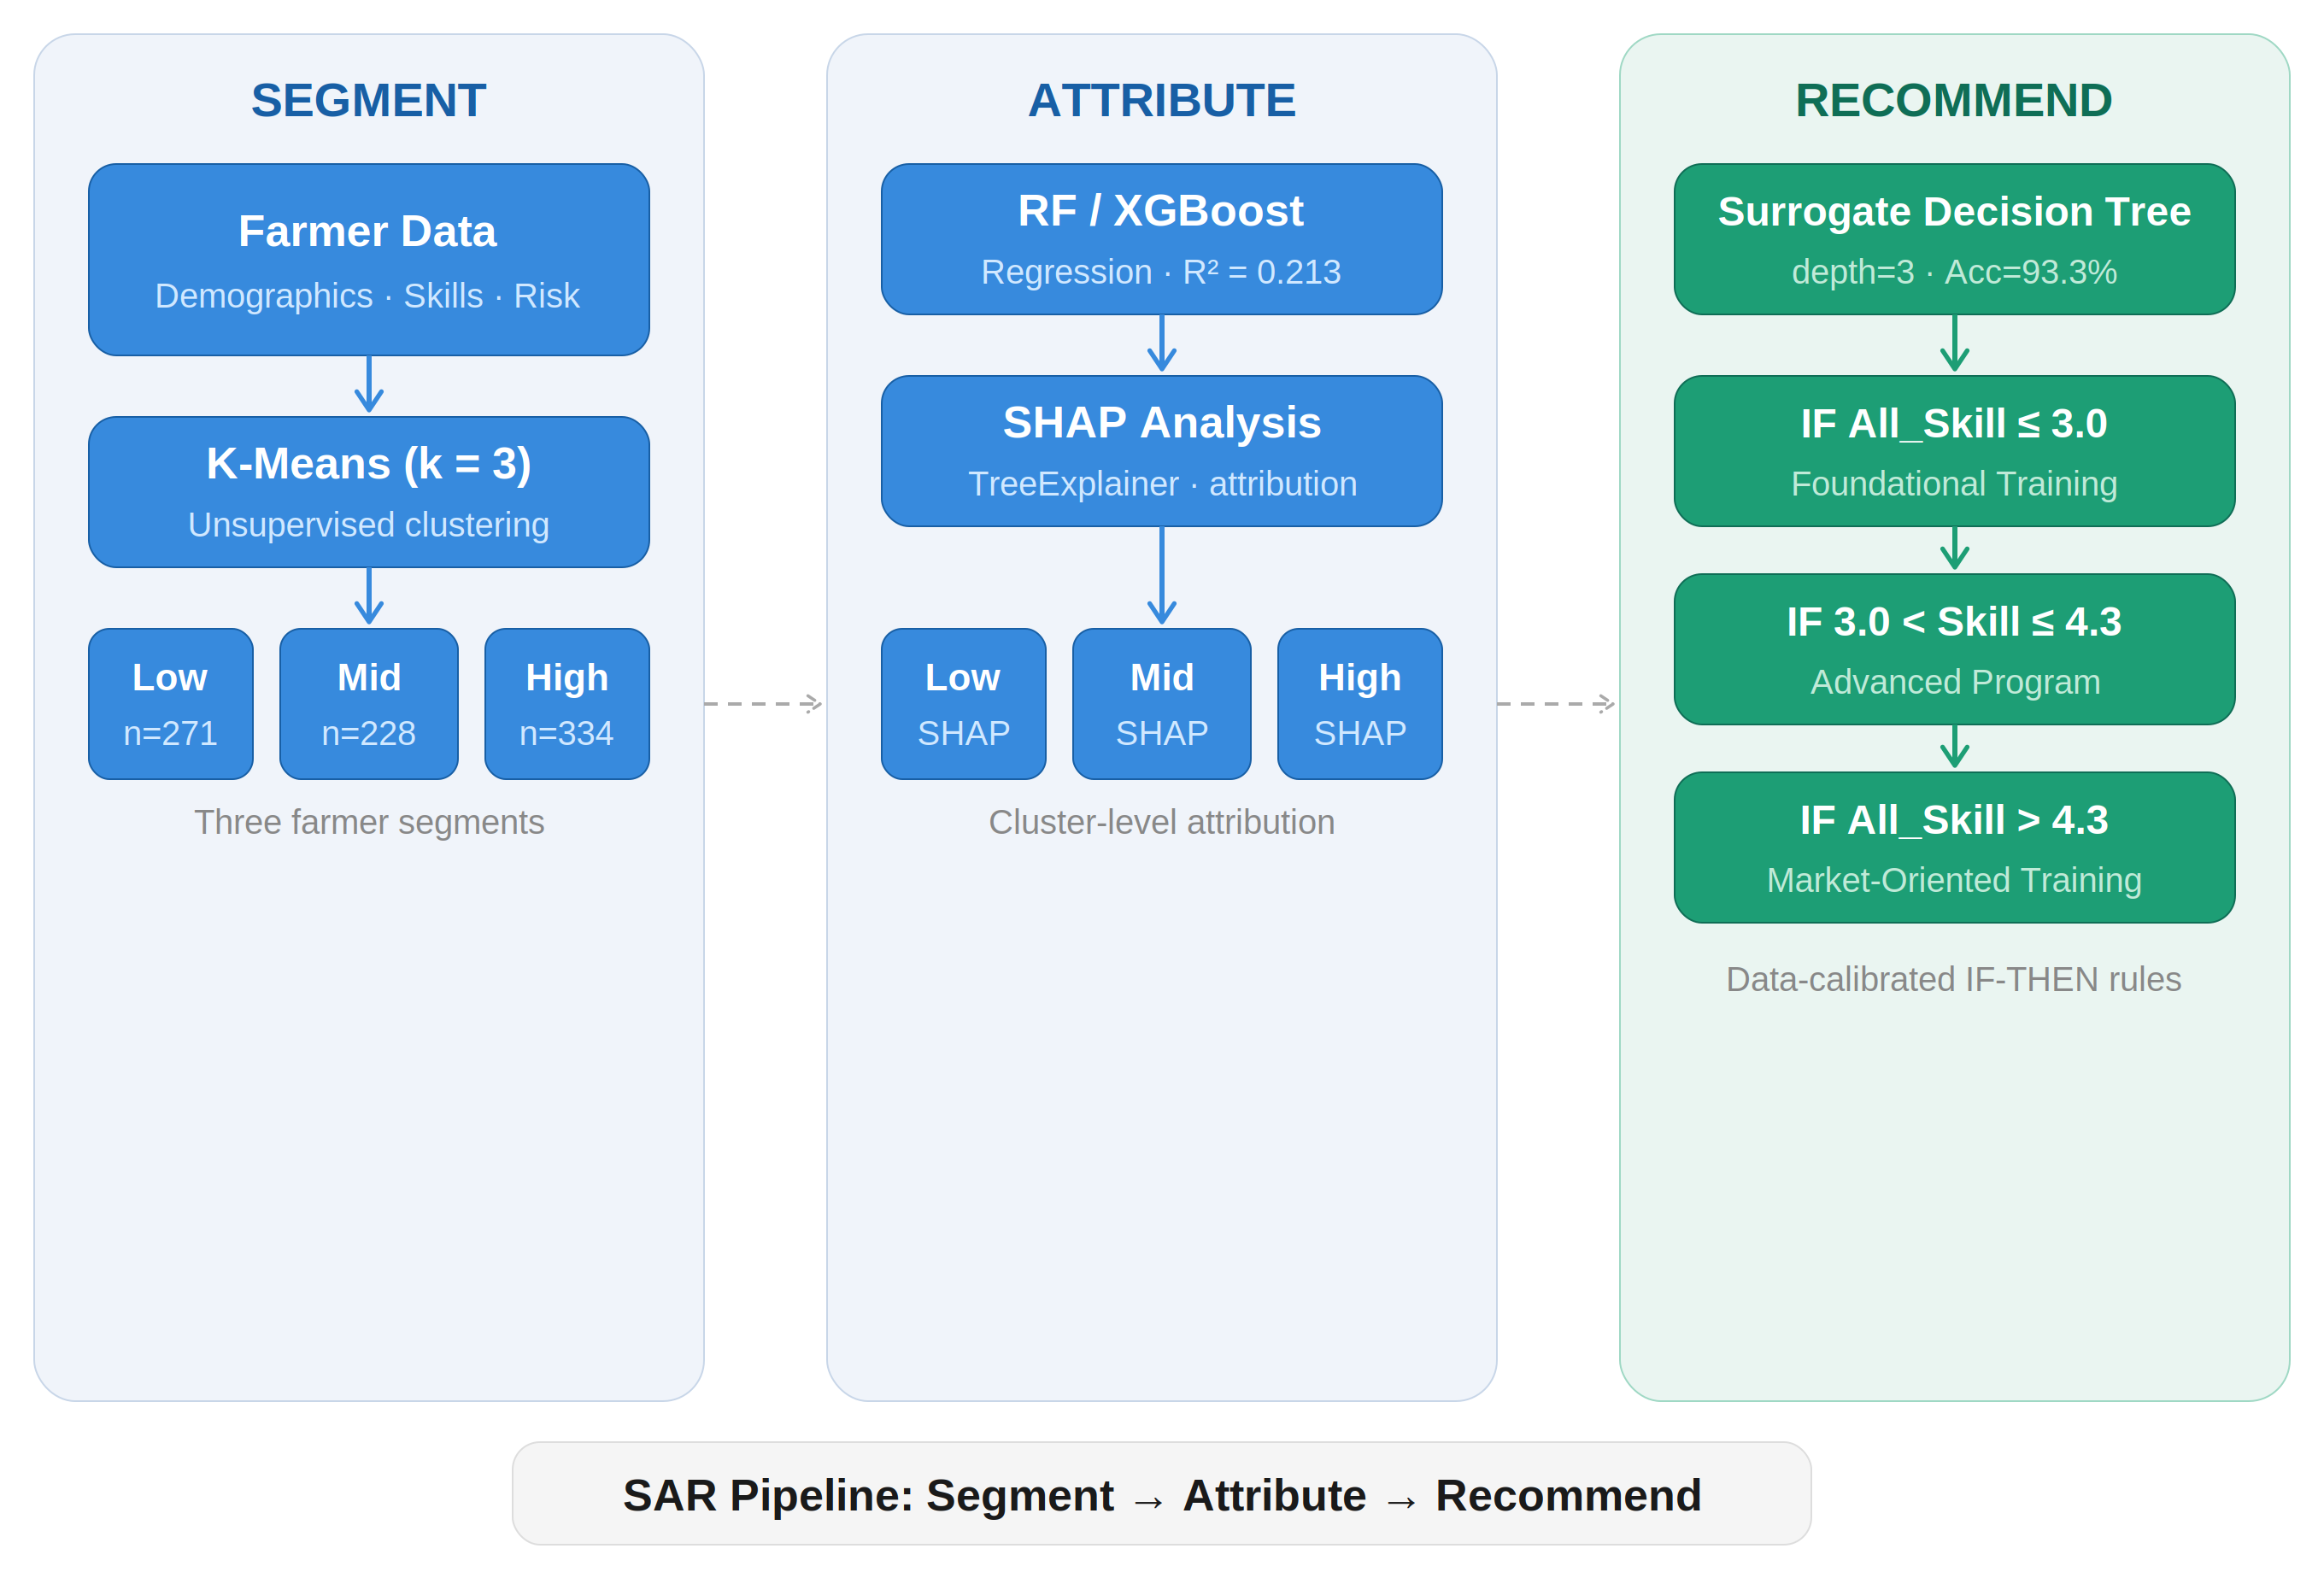
\includegraphics[width=\textwidth]{figures/fig1_framework.png}
\caption{SAR framework: three-stage pipeline (Segment, Attribute, Recommend) for interpretable allocation.}
\label{fig:framework}
\end{figure*}

\begin{figure}[htbp]
\centering

\includegraphics[width=\columnwidth]{figures/fig_elbow_silhouette.png}
\caption{Cluster validity across $k = 2$--$8$: Elbow, Silhouette, Calinski--Harabasz, and Davies--Bouldin.
At $k = 3$: Silhouette $= 0.185$, CH $= 202.67$, DB $= 1.835$.}
\label{fig:elbow}
\end{figure}

\begin{figure}[htbp]
\centering

\includegraphics[width=\columnwidth]{figures/fig2_clusters_new.png}
\caption{Population segmentation via K-Means ($k = 3$) in PCA space. Three clusters show different profiles.}
\label{fig:clusters}
\end{figure}

\begin{figure}[htbp]
\centering
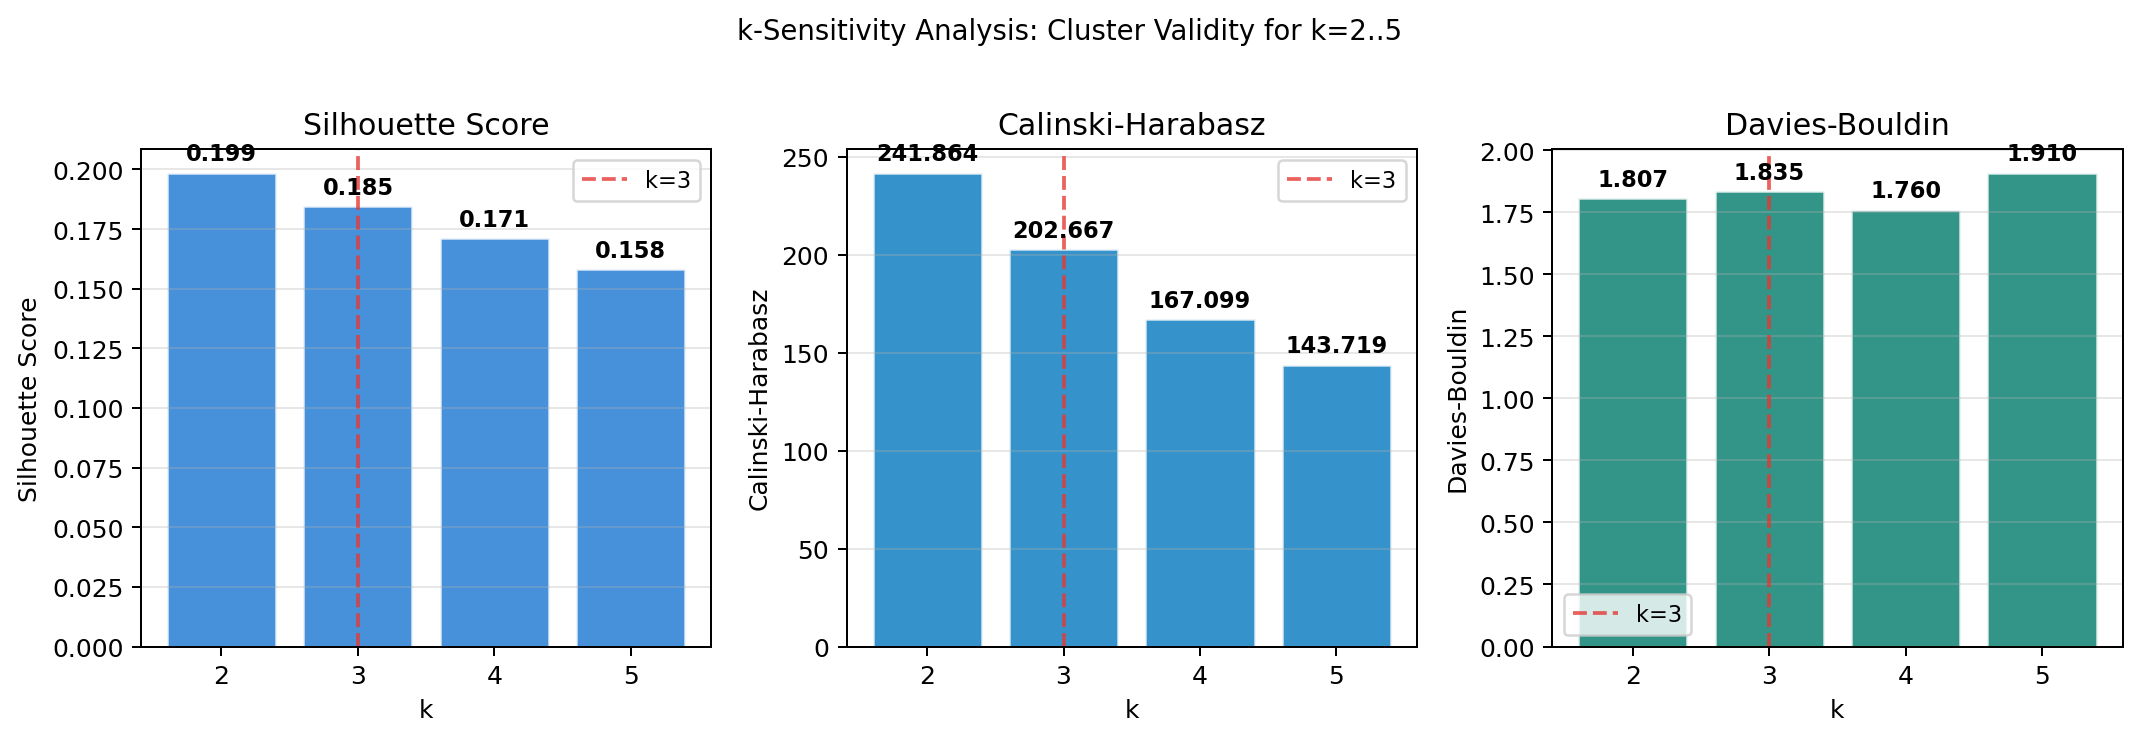
\includegraphics[width=\columnwidth]{figures/fig_k_sensitivity.png}
\caption{K-sensitivity analysis: validity indices for $k = 2$--$5$. Segment structure remains consistent.
values of $k$, supporting the robustness of the three-segment solution.}
\label{fig:sensitivity}
\end{figure}

\begin{figure}[htbp]
\centering
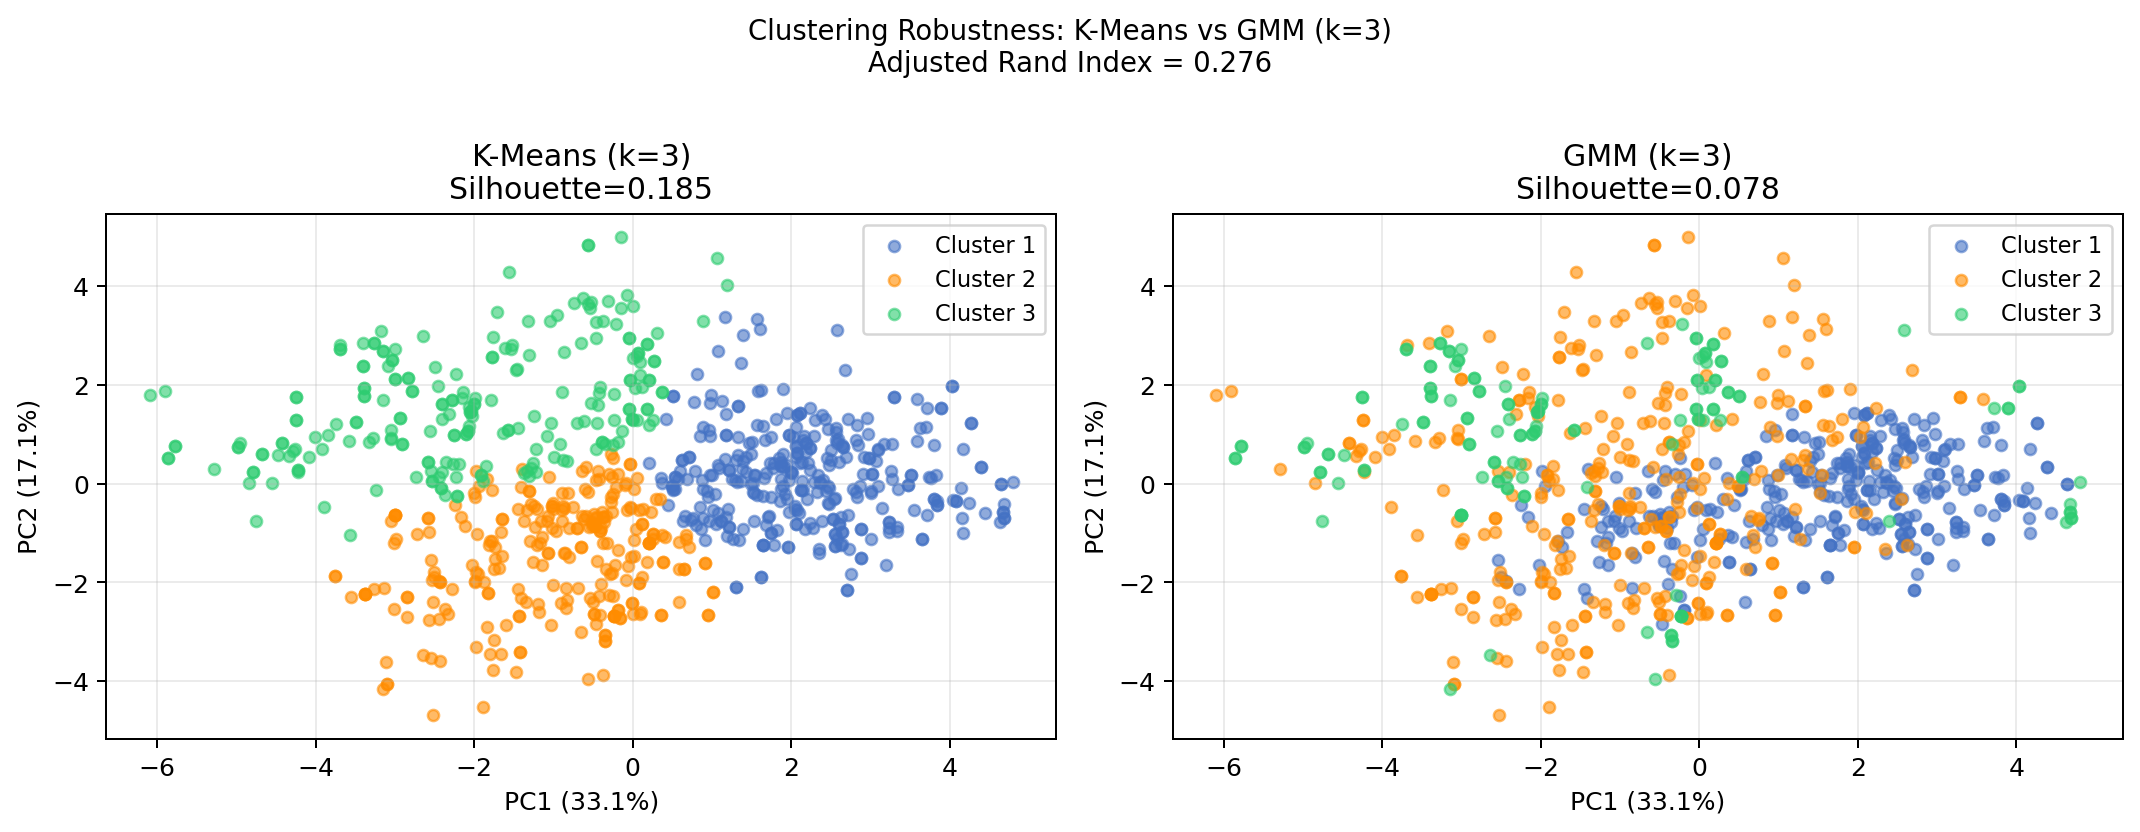
\includegraphics[width=\columnwidth]{figures/fig_gmm_robustness.png}
\caption{Clustering robustness: K-Means versus GMM ($k = 3$). Adjusted Rand Index = 0.28.
K-Means produces more balanced and interpretable segment groupings
than GMM in this Likert-scale dataset.}
\label{fig:gmm}
\end{figure}

\begin{figure}[htbp]
\centering

\includegraphics[width=\columnwidth]{figures/fig3_importance_new.png}
\caption{Global SHAP importance across all observations ($n = 833$). \texttt{All\_Skill} is the top driver.}
%\caption{Global SHAP importance across all observations ($n = 833$). All_Skill is the top driver.}
\label{fig:importance}
\end{figure}

\begin{figure}[htbp]
\centering
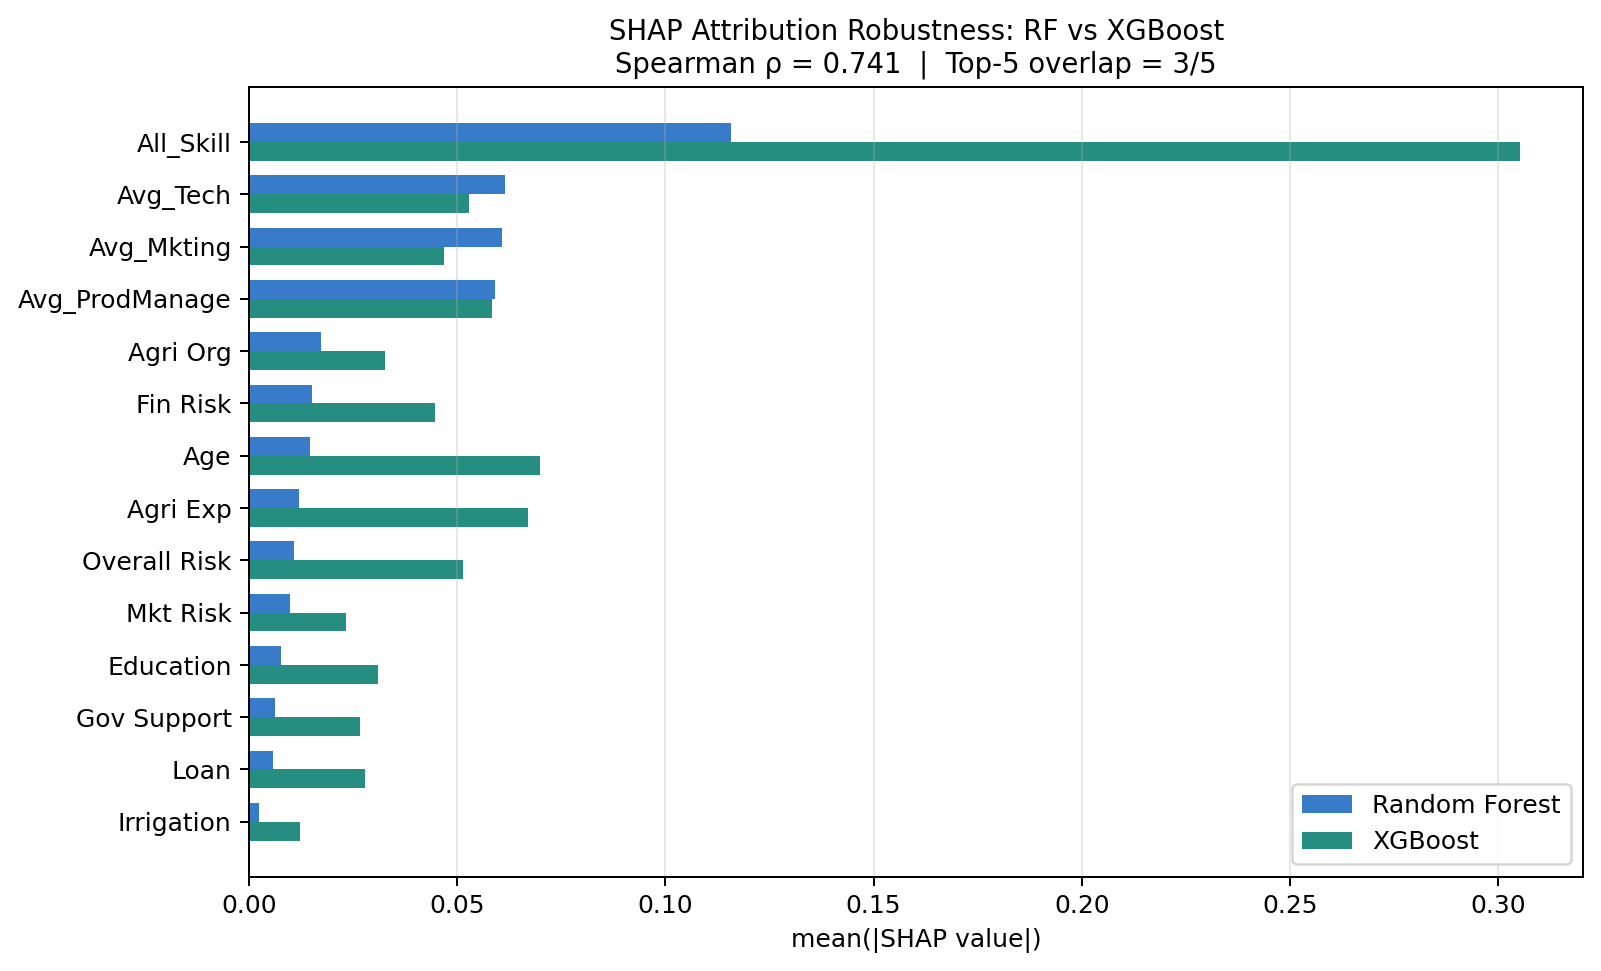
\includegraphics[width=\columnwidth]{figures/fig_shap_robustness.png}
\caption{SHAP robustness: RF vs. XGBoost ranking agreement ($\rho = 0.793$, $p < 0.001$).}
\label{fig:robustness}
\end{figure}

\begin{figure}[htbp]
\centering
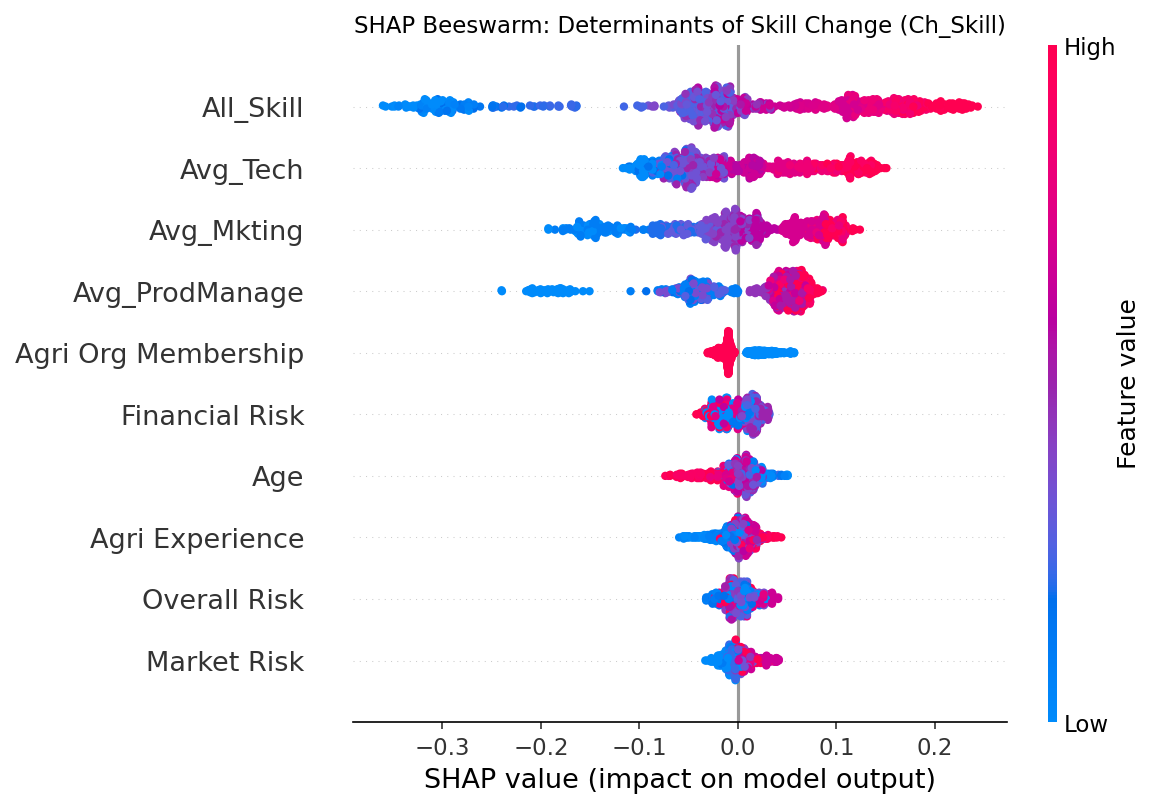
\includegraphics[width=\columnwidth]{figures/fig4_shap_new.png}
\caption{SHAP beeswarm: feature contribution patterns ($n = 833$). Red = high, blue = low values.}
\label{fig:shap}
\end{figure}

\begin{figure*}[htbp]
\centering

\includegraphics[width=\textwidth]{figures/fig4b_cluster_shap_new.png}
\caption{Cluster-stratified SHAP: three segments show different feature patterns ($n = 271, 228, 334$).
systematically across segments.}
\label{fig:clusterShap}
\end{figure*}

\begin{figure*}[htbp]
\centering

\includegraphics[width=\textwidth]{figures/fig5_rules_new.png}
\caption{Surrogate decision tree (depth 3): in-sample accuracy 93.3% ($n = 817$), held-out 91.4%.
Node labels show the splitting feature, threshold, sample count,
and class distribution.}
\label{fig:rules}
\end{figure*}

%%─────────────────────────────────────────────────────────────────────────────
\section{Discussion}
%%─────────────────────────────────────────────────────────────────────────────

\subsection{Predictive Performance in Context}

The Random Forest achieves $R^{2} = 0.283$ under farmer-level GroupKFold
cross-validation, outperforming both linear and ridge regression baselines
($R^{2} = 0.257$). This improvement reflects non-linear threshold effects and
feature interactions that additive models cannot capture. Modest absolute
$R^{2}$ values are expected in observational studies of human learning, where
skill change depends heavily on motivation, engagement, and trainer quality
\citep{davis2012}.

Within SAR, the Random Forest serves a structural rather than a purely
predictive role. \citet{lundberg2020} show that SHAP attributions can remain
stable and informative at moderate predictive accuracy, provided the model
captures meaningful data structure. This condition is supported here by
cross-model attribution agreement ($\rho = 0.793$,
Fig.~\ref{fig:robustness}). Decision logic in SAR is implemented through the
surrogate rule structure, not through point predictions. The framework’s
analytical value therefore depends on the consistency of attribution and rule
extraction rather than short-term forecasting precision.

\subsection{Segment-Specific Drivers and Negative Skill Change}

Cluster-level SHAP shows that the determinants of skill change vary
systematically across segments, a pattern that cannot be recovered from global
feature importance alone. Baseline skill (\texttt{All\_Skill}) is the dominant
contributor in all segments, consistent with human capital theory
\citep{feder1985,davis2012}.

The negative mean skill change in the Low-skill ($-0.233$) and Moderate-skill
($-0.105$) segments has two likely explanations. First, regression-to-the-mean:
farmers with the lowest initial scores are more susceptible to downward
variation in repeated assessments \citep{davis2012}. Second, the voluntary
structure of the program leads to lower participation among Low-skill farmers
(28.8\%) compared with High-skill farmers (69.8\%). Observed trajectories in
lower-skill segments therefore partly reflect farmers with limited or no
training exposure \citep{anderson2004}.

In the High-skill segment, marketing skill (\texttt{Avg\_Mkting}) becomes more
important relative to other predictors. This suggests that market-oriented
competencies are the binding constraint at higher skill levels, pointing toward
advanced market-integration training for this group.

\subsection{Decision Rule Validity and Generalisation}

The surrogate tree achieves 93.3\% in-sample accuracy. Farmer-level held-out
validation (80/20 split, Option~B) yields 91.4\% accuracy on unseen farmers, and
5-fold GroupKFold cross-validation yields 95.3\% $\pm$ 2.5\%. The consistent
performance across all three approaches confirms that the decision rules
generalise beyond the training data.

The two-stage extraction process—SHAP for feature selection and a surrogate tree
for threshold calibration—ensures that the rules are both theoretically grounded
and empirically calibrated \citep{molnar2022}. Key thresholds correspond closely
to proficiency distinctions within Thailand’s Smart Farmer program, supporting
the institutional plausibility of the results. Following \citet{rudin2019}, the
surrogate rules should be interpreted as structured decision aids rather than
exact reconstructions of the Random Forest process.

\subsection{Operational Deployment Scenario}

SAR can be implemented as a lightweight, rule-based decision tool. A typical
workflow involves four steps:
\begin{enumerate}
  \item Recording a farmer’s baseline profile (demographics, skills, resources)
  \item Assigning the farmer to a segment via K-Means
  \item Applying segment-specific surrogate rules
  \item Generating a structured training recommendation
\end{enumerate}

This process does not require direct model interaction and can be implemented
through a rule-based interface. The explicit rule structure supports
transparency and auditability, which are key requirements in public-sector
extension systems.

Three structural insights emerge from the analysis:
\begin{enumerate}
  \item Pre-training capability is the dominant driver of learning outcomes
  across all segments.
  \item Binding constraints differ by segment: production and education
  limitations dominate at lower skill levels, while marketing competencies matter
  more for advanced farmers.
  \item Uniform training structures are poorly matched to heterogeneous
  populations, as shown by negative or negligible skill change in the Low- and
  Moderate-skill segments.
\end{enumerate}

\subsection{Limitations}

All findings are associative. Causal interpretation requires randomised or
quasi-experimental designs. The segmentation structure and thresholds are
calibrated to the Thai Smart Farmer population and require recalibration for
other contexts. Low Silhouette scores indicate soft cluster boundaries; segments
should be interpreted as practical groupings rather than sharply separated
types. Held-out validation confirms generalisation, but further prospective
field validation is needed before operational deployment. Following
\citet{rudin2019}, the surrogate model approximates the Random Forest and should
not be treated as an exact replica.

%%─────────────────────────────────────────────────────────────────────────────
\section{Conclusion}
%%─────────────────────────────────────────────────────────────────────────────

This study presents an explainable AI-based decision support system for the
precision allocation of agricultural skill development programs, using data from
$n = 833$ farmers in Thailand's Smart Farmer initiative.

By integrating K-Means segmentation, Random Forest modelling, and SHAP
explainability within the SAR architecture, the framework provides a deployable
and auditable pathway from farmer-level data to structured training
recommendations. Baseline skill level, production management competency, and
educational attainment are the primary contributors to training outcomes, with
their relative importance varying across segments. Cluster-level SHAP analysis,
validated through cross-model agreement with XGBoost ($\rho = 0.793$), shows
that global feature importance alone is insufficient for precision training
design.

The main methodological contribution is the integration of cluster-conditioned
explainability with surrogate decision tree extraction. This approach translates
complex model structure into transparent IF--THEN rules that are interpretable
and aligned with observed data patterns. The surrogate rules generalise well
beyond the training data, as confirmed by held-out accuracy (91.4\%) and 5-fold
cross-validated accuracy (95.3\% $\pm$ 2.5\%).

Rather than focusing on predictive accuracy alone, SAR prioritises structural
consistency, interpretability, and operational feasibility. It offers a
practical foundation for modernising agricultural extension systems through
explainable AI.

Future work should focus on (i) expanded out-of-sample validation of surrogate
rules, (ii) quasi-experimental assessment of training effects, and (iii)
integration with real-time agricultural data systems. Progress on these fronts
will strengthen the inferential credibility and practical scalability of
AI-supported agricultural extension \citep{yang2025,zhang2026}.


%%─────────────────────────────────────────────────────────────────────────────
\section*{Acknowledgements}
This study was supported by USAID through Michigan State University and the
Department of Agriculture and Resource Economics in the Faculty of Economics,
Kasetsart University. Additional support for the data analysis and machine
learning components was provided by the Research and Development Institute,
Bansomdejchaopraya Rajabhat University. The author is grateful to all survey
respondents for their cooperation. The author also thanks Professor Mywish
Maredia of Michigan State University for her guidance, Ms.\ Jumtip for her work
on questionnaire design, data collection, and impact evaluation, and the
officers in the Farmer Development Division of the Department of Agricultural
Extension for providing participant information.

\section*{Funding}
This study received support from USAID through Michigan State University and the
Department of Agriculture and Resource Economics, Faculty of Economics,
Kasetsart University. Additional funding for data analysis and machine learning
was provided by the Research and Development Institute, Bansomdejchaopraya
Rajabhat University, through its academic promotion program.

\section*{Ethics Statement}
This study was reviewed and exempted by the Kasetsart University Research Ethics
Committee (KUREC-SSR67/056). All data were anonymised prior to analysis.

\section*{Data Availability}
The anonymised dataset and analysis code are available from the corresponding
author upon reasonable request, subject to the data-sharing agreement with the
Department of Agricultural Extension, Thailand.

\section*{Declaration of Competing Interest}
The authors declare no competing interests.

\section*{Author Contributions}
Kitti: Conceptualisation, Methodology, Machine Learning Analysis, Data Analysis,
Writing -- Original Draft.\\
Jumtip: Questionnaire Design, Survey Data Collection, Difference-in-Difference
(DID) Impact Evaluation, Data Curation.

\section*{Declaration of Generative AI and AI-assisted technologies}
During the preparation of this manuscript, the authors used Microsoft Copilot to
assist with language refinement and clarity, and used Claude to support the
creation of the graphical abstract and illustrative framework figures. All
analytical decisions, interpretations, and substantive content were developed by
the authors. The authors reviewed, edited, and verified all generated material
and take full responsibility for the final content of the article.

%%─────────────────────────────────────────────────────────────────────────────
\begin{thebibliography}{35}
\expandafter\ifx\csname natexlab\endcsname\relax
  \def\natexlab#1{#1}\fi
\providecommand{\url}[1]{\texttt{#1}}
\providecommand{\href}[2]{#2}
\providecommand{\path}[1]{#1}
\providecommand{\doi}[1]{\href{https://doi.org/#1}{#1}}

\bibitem[{MacQueen(1967)}]{macqueen1967}
MacQueen, J., 1967.
Some methods for classification and analysis of multivariate observations.
In: Proc.\ 5th Berkeley Symposium on Mathematical Statistics and Probability,
vol.\ 1, pp.\ 281--297.

\bibitem[{Feder et~al.(1985)}]{feder1985}
Feder, G., Just, R.E., Zilberman, D., 1985.
Adoption of agricultural innovations in developing countries: A survey.
Economic Development and Cultural Change 33, 255--298.

\bibitem[{Rousseeuw(1987)}]{rouseeuw1987}
Rousseeuw, P.J., 1987.
Silhouettes: A graphical aid to the interpretation and validation of
cluster analysis.
Journal of Computational and Applied Mathematics 20, 53--65.

\bibitem[{Breiman(2001)}]{breiman2001}
Breiman, L., 2001.
Random forests.
Machine Learning 45, 5--32.

\bibitem[{Anderson and Feder(2004)}]{anderson2004}
Anderson, J.R., Feder, G., 2004.
Agricultural extension: Good intentions and hard realities.
World Bank Research Observer 19, 41--60.

\bibitem[{Davis and Franzel(2012)}]{davis2012}
Davis, K., Franzel, S., 2012.
Principles for designing and implementing agricultural extension programs.
Journal of Agricultural Education and Extension 18, 249--263.

\bibitem[{Chen and Guestrin(2016)}]{chen2016}
Chen, T., Guestrin, C., 2016.
XGBoost: A scalable tree boosting system.
In: Proc.\ 22nd ACM SIGKDD, pp.\ 785--794.

\bibitem[{Lundberg and Lee(2017)}]{lundberg2017}
Lundberg, S.M., Lee, S.I., 2017.
A unified approach to interpreting model predictions.
Advances in Neural Information Processing Systems (NeurIPS).

\bibitem[{Ghosal et~al.(2018)}]{ghosal2018}
Ghosal, S., Blystone, D., Singh, A.K., Ganapathysubramanian, B.,
  Singh, A., Sarkar, S., 2018.
An explainable deep machine vision framework for plant stress phenotyping.
PNAS 115, 4613--4618.

\bibitem[{Kamilaris and Prenafeta-Boldu(2018)}]{kamilaris2018}
Kamilaris, A., Prenafeta-Boldu, F.X., 2018.
Deep learning in agriculture: A survey.
Computers and Electronics in Agriculture 147, 70--90.

\bibitem[{Liakos et~al.(2018)}]{liakos2018}
Liakos, K.G., Busato, P., Moshou, D., Pearson, S., Bochtis, D., 2018.
Machine learning in agriculture: A review.
Sensors 18, 2674.

\bibitem[{Guidotti et~al.(2019)}]{guidotti2019}
Guidotti, R., Monreale, A., Ruggieri, S., Turini, F., Giannotti, F.,
  Pedreschi, D., 2019.
A survey of methods for explaining black box models.
ACM Computing Surveys 51(5), 93.

\bibitem[{Rudin(2019)}]{rudin2019}
Rudin, C., 2019.
Stop explaining black box machine learning models for high stakes
decisions and use interpretable models instead.
Nature Machine Intelligence 1, 206--215.

\bibitem[{Arrieta et~al.(2020)}]{arrieta2020}
Arrieta, A.B., Diaz-Rodriguez, N., Del Ser, J., et~al., 2020.
Explainable artificial intelligence (XAI): Concepts, taxonomies,
opportunities and challenges.
Information Fusion 58, 82--115.

\bibitem[{Lundberg et~al.(2020)}]{lundberg2020}
Lundberg, S.M., Erion, G., Chen, H., DeGrave, A., Prutkin, J.M.,
  Nair, B., Katz, R., Himmelfarb, J., Bansal, N., Lee, S.I., 2020.
From local explanations to global understanding with explainable AI
for trees.
Nature Machine Intelligence 2, 56--67.

\bibitem[{Linardatos et~al.(2021)}]{linardatos2021}
Linardatos, P., Papastefanopoulos, V., Kotsiantis, S., 2021.
Explainable AI: A review of machine learning interpretability methods.
Entropy 23(1), 18.

\bibitem[{Ryo(2022)}]{ryo2022}
Ryo, M., 2022.
Explainable artificial intelligence and interpretable machine learning
for agricultural data analysis.
Artificial Intelligence in Agriculture 6, 257--265.

\bibitem[{Hossain et~al.(2022)}]{hossain2022cattle}
Hossain, M.E., Kabir, M.A., Zheng, L., Swain, D.L., McGrath, S.,
  Medway, J., 2022.
A systematic review of machine learning techniques for cattle
identification.
Computers and Electronics in Agriculture 198, 107090.

\bibitem[{Molnar(2022)}]{molnar2022}
Molnar, C., 2022.
Interpretable Machine Learning: A Guide for Making Black-Box Models
Explainable.
\url{https://christophm.github.io/interpretable-ml-book/}

\bibitem[{Ennaji et~al.(2023)}]{ennaji2023nutrient}
Ennaji, O., Vergütz, L., El Allali, A., 2023.
Machine learning in nutrient management: A review.
Computers and Electronics in Agriculture 205, 107623.

\bibitem[{Ghazal et~al.(2024)}]{ghazal2024survey}
Ghazal, S., Munir, A., Qureshi, W.S., 2024.
Computer vision in smart agriculture and precision farming.
Computers and Electronics in Agriculture 214, 108486.

\bibitem[{Omaye et~al.(2024)}]{omaye2024disease}
Omaye, J.D., Ogbuju, E., Ataguba, G., Jaiyeoba, O., Aneke, J.,
  Oladipo, F., 2024.
Cross-comparative review of machine learning for plant disease detection.
Computers and Electronics in Agriculture 212, 108345.

\bibitem[{Wonggasem et~al.(2024)}]{wonggasem2024}
Wonggasem, K., Chakranon, P., Wongchaisuwat, P., 2024.
Automated quality inspection of baby corn using image processing
and deep learning.
Artificial Intelligence in Agriculture 11, 61--69.

\bibitem[{Li et~al.(2025)}]{li2025llm}
Li, H., Wu, H., Li, Q., Zhao, C., 2025.
A review on enhancing agricultural intelligence with large language
models.
Artificial Intelligence in Agriculture 17, 100--125.

\bibitem[{Yang et~al.(2025)}]{yang2025}
Yang, H., et~al., 2025.
AI-driven aquaculture: A review of technological innovations and
sustainable impacts.
Artificial Intelligence in Agriculture 15, 508--525.

\bibitem[{Zhang et~al.(2026)}]{zhang2026}
Zhang, T., et~al., 2026.
Empowering Chinese medicinal agriculture through AI-driven technologies:
A comprehensive review.
Artificial Intelligence in Agriculture. \textit{In press.}

\end{thebibliography}

\end{document}